
% Muon events, threshold analysis
Analysis of LED events can only be applied on the four extra top modules. To determine the stability of the total \mvs, ageing of all modules must be investigated. In this chapter, the muon-events are selected and analysed. Additionally, the effective threshold of each module is determined using an independent method, which allows to estimate the change of the detection efficiency of the modules.

\section{Analysis of muon events}

\subsection{Selection of muon-veto data}
All the data from Run70 (Aug 2010) to Run138 (Mar 2017) are investigated in the following analysis. Since the goal is to analyse the stability of muon detection in modules, several cuts are applied on the data to ensure a proper acquisition condition of the system over the investigated time period and to decrease background events.\\
First, data taken when the \mvs{} was not fully closed are rejected. As described in sec.\,\ref{sec:muon-setup}, two lasers measure the position of the upper part of the muon-veto every 15 minutes. Time periods when the gap size deviates more than 5 cm from the closed configuration are cut, since the \mvs{} is either fully closed or fully opened. When the system is opened, the detection efficiency of through-going muons decreases and the background rate increases largely, which will lead to an increase of low energy events.

When the \mvs{} is closed, most muons go through at least 2 modules. Therefore a coincidence in 2 distinct modules is required for selecting muon events. An energy deposit with full information in each module is required, i.e.\,both TDCs and ADCs must have non-zero values. It respectively reduces events caused by secondary particles or radioactive backgrounds as they mostly deposit less energy than muons. By applying this cut criterium, the event rate in one module is reduced to the order of $\SI{10}{events/day}$.

\subsection{HV stability}
The HV applied on the modules over the investigated time period from year 2010 and 2017 are first analysed. During the time period, the HV of 25 scintillator modules are not changed. In March 2013, the HV on 21 modules were slightly increased to compensated the decrease of event rate due to the ageing effect. For example in Module 32, the HVs on the both PMT groups were increased from -1700\,V to -1710\,V (see fig.\,\ref{fig:HV_32}).

\begin{figure}[htb!]
  \centering
  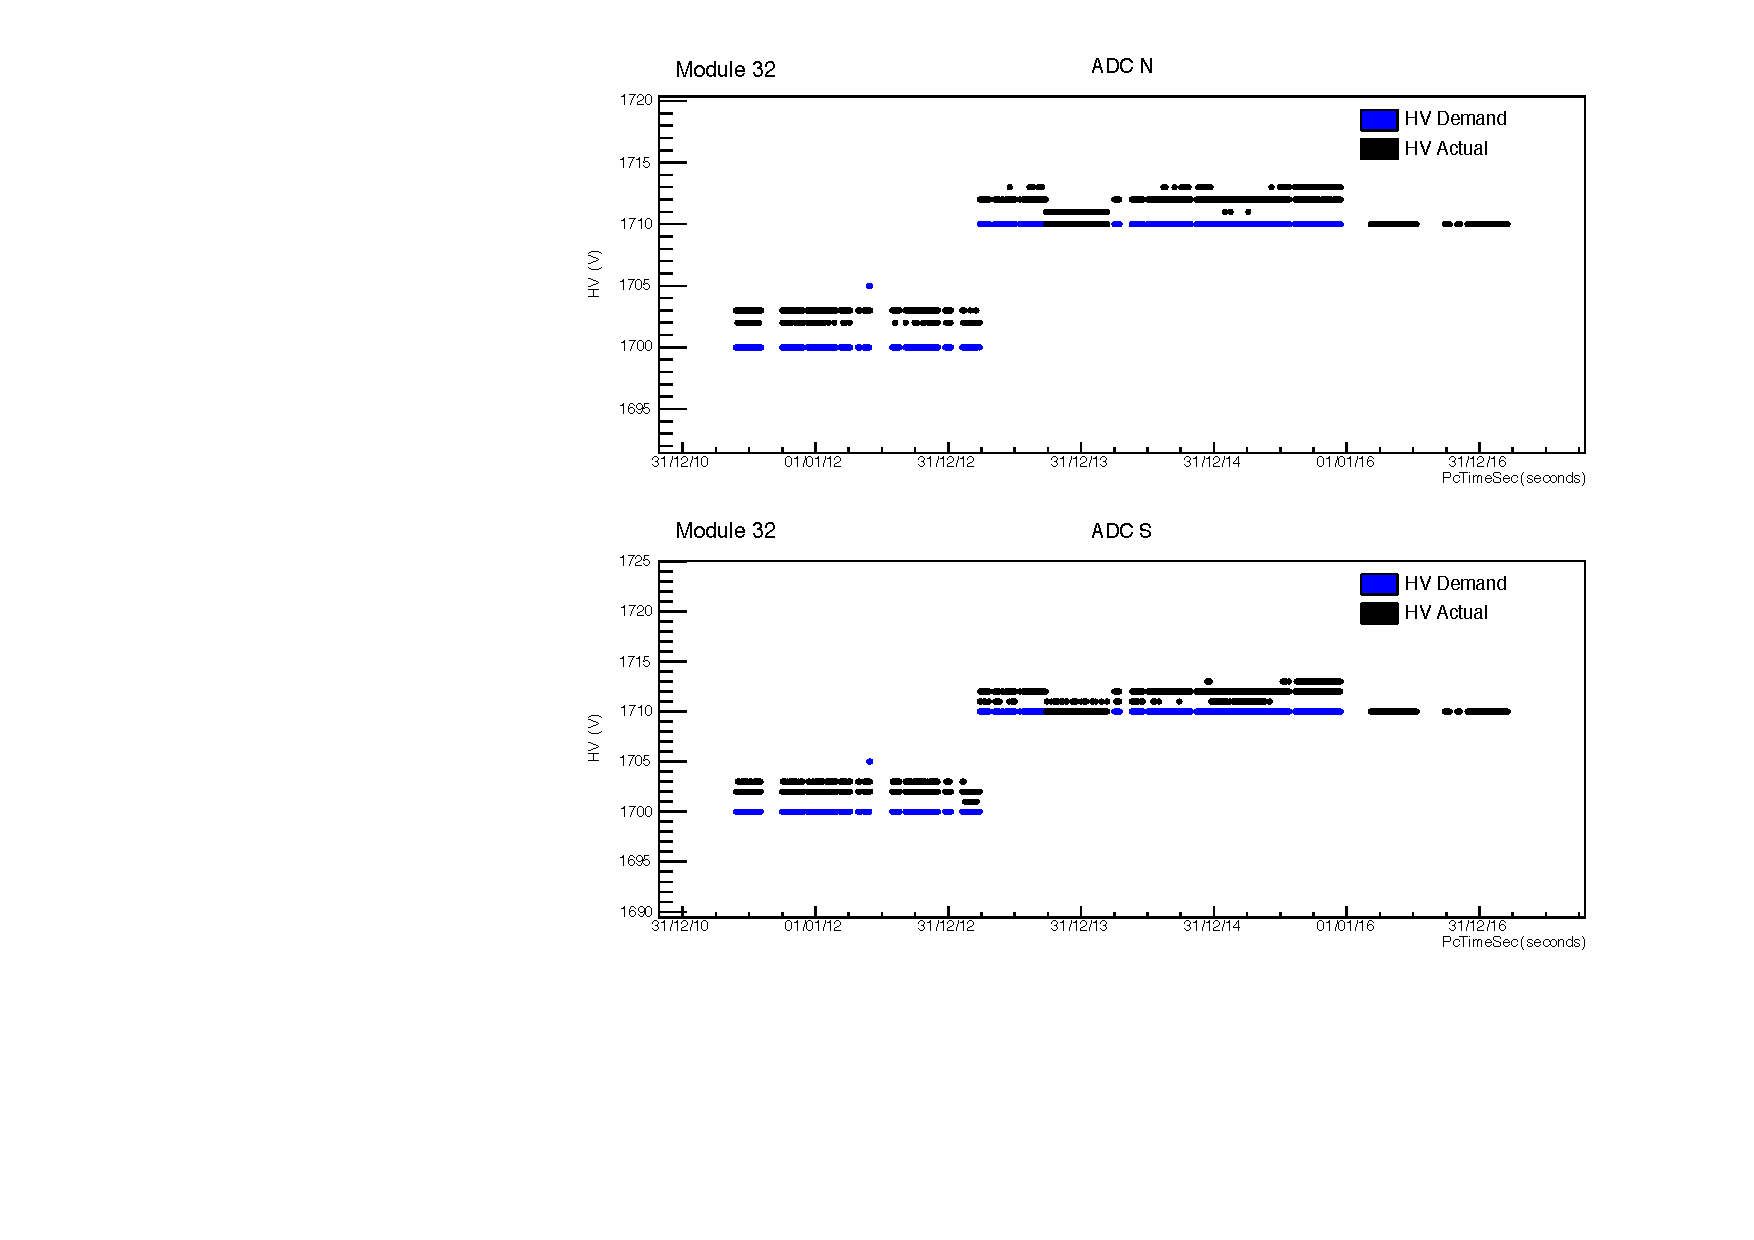
\includegraphics[width=0.9\textwidth{}]{./fig/HVPlot_M32.pdf}
  \caption{HV applied on M32 from year 2010 to 2017. The HV applied on the module is negative and the plot shows the absolute value of the HV. The blue points are the set value of the HV and the black points are the actual measured HV. In March 2013, the set HV was increased from -1700\,V to -1710\,V for both PMT groups.}
  \label{fig:HV_32}
\end{figure}

For all modules, the result shows that the measured HV values only have small fluctuation from the demand values. Therefore, the HV is stable for all modules over the total time period.

\subsection{Data analysis}
As mentioned in section \ref{sec:muon-working}, the spectrum of muon energy deposit in modules can be described by a Landau distribution. The ADC values of muon events in a given time period are fitted with a Landau distribution and the obtained MPVs in different time periods are used to analyse the long term behaviour of the \mvs.  Fig.\,\ref{fig:Landau_M6} shows an example of the Landau fit. Since the muon event rate is low, the obtained ADC values in a two months period are combined to perform each fit.

\begin{figure}[ht]
  \centering
  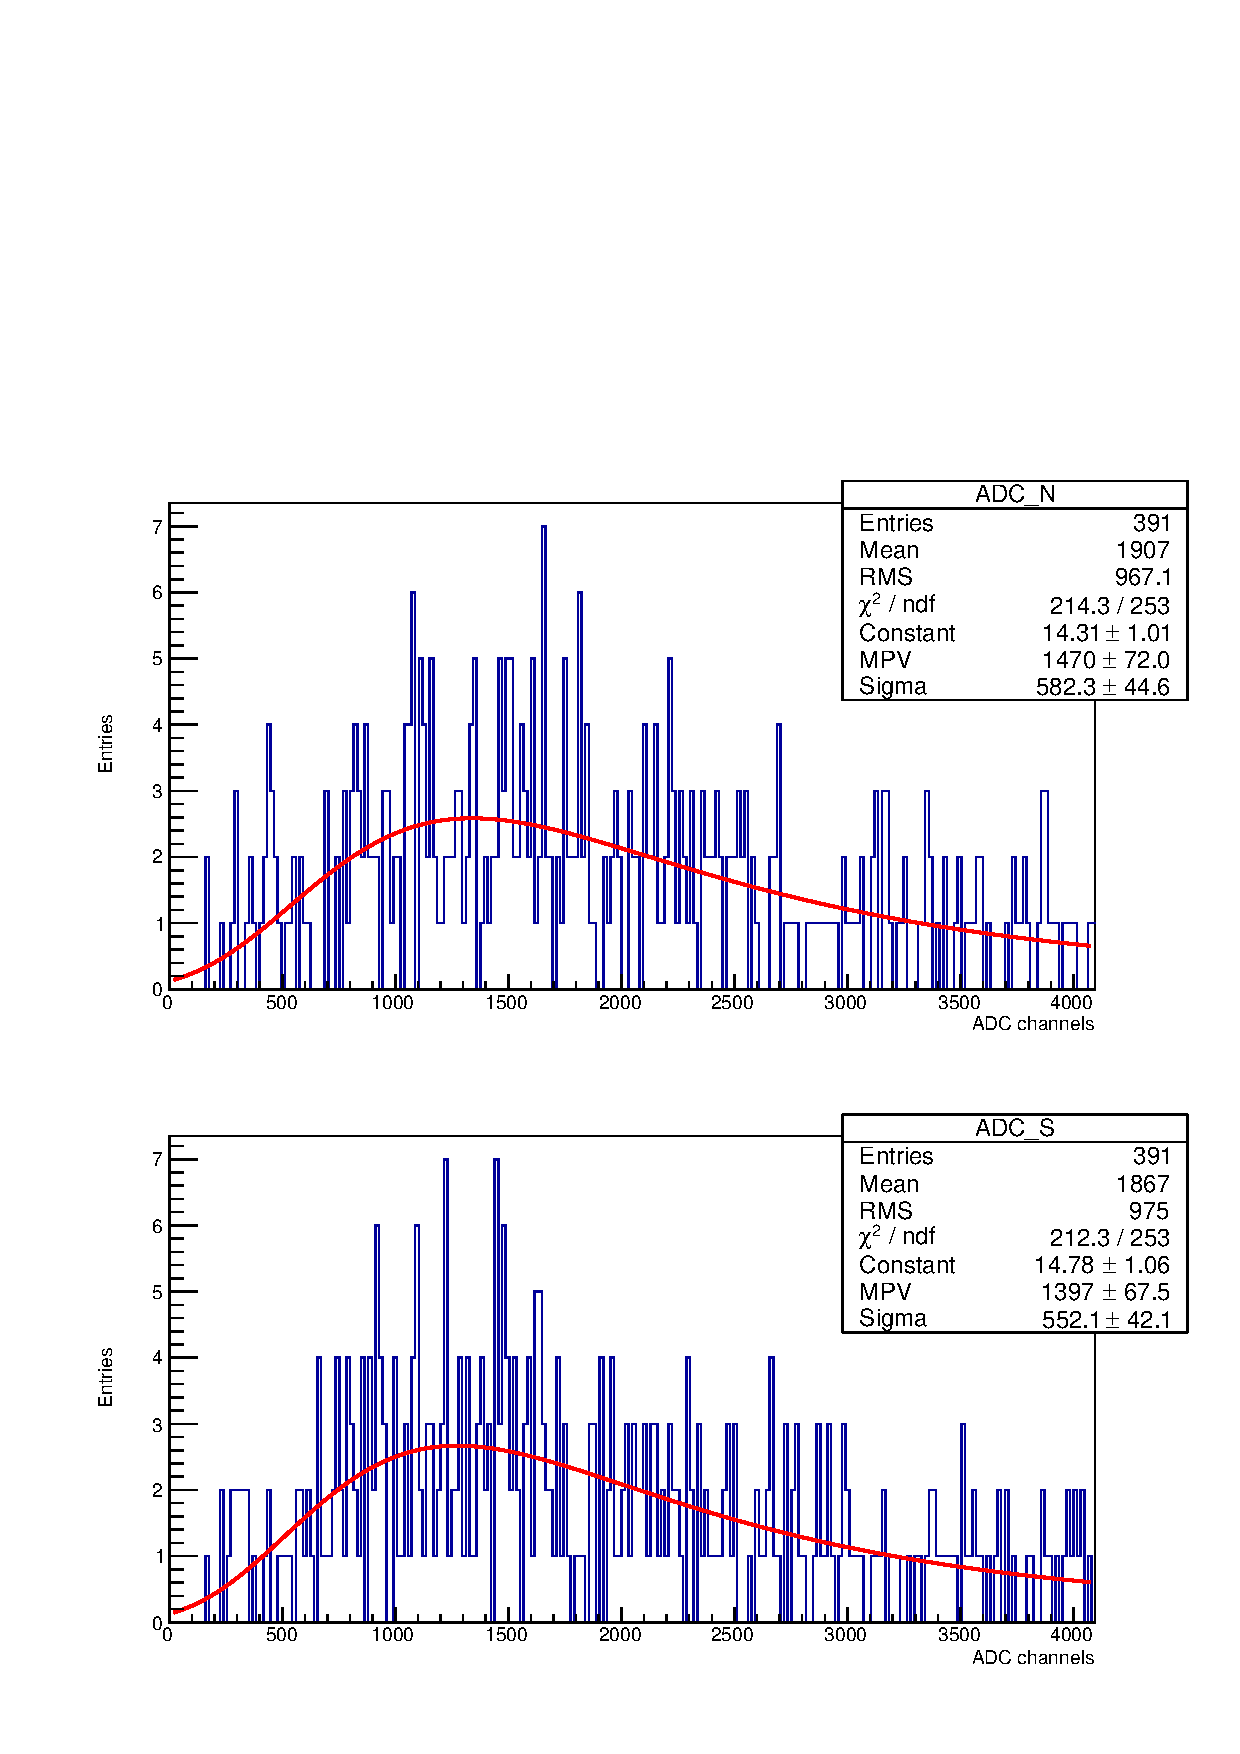
\includegraphics[width=0.6\textwidth{}]{./fig/LandauFitM6.pdf}
  \caption{Example of a Landau fit in M6. The fit uses a log likelihood method in ROOT. The muon-induced events are collected over a period of two months.}
  \label{fig:Landau_M6}
\end{figure}

The MPVs obtained from the Landau fit are plotted over time (see fig.\ \ref{fig:MPV}). Some time periods with too few entries due to system shutoffs are excluded, since no reliable Landau fit can be performed. It is to be noticed that the data points have rather large uncertainty, which is partially due to the smeared spectrum. As explained before, the light output is strongly position dependent and decreases exponentially with the path length from the interaction point to the PMT group. Furthermore, there are some sudden changes of the MPVs. The reason could be the restart of the \mvs{} after operations and unstable data acquisition.

\begin{figure}[hp!]
  \centering
  \begin{subfigure}{0.6\linewidth}
    \centering
    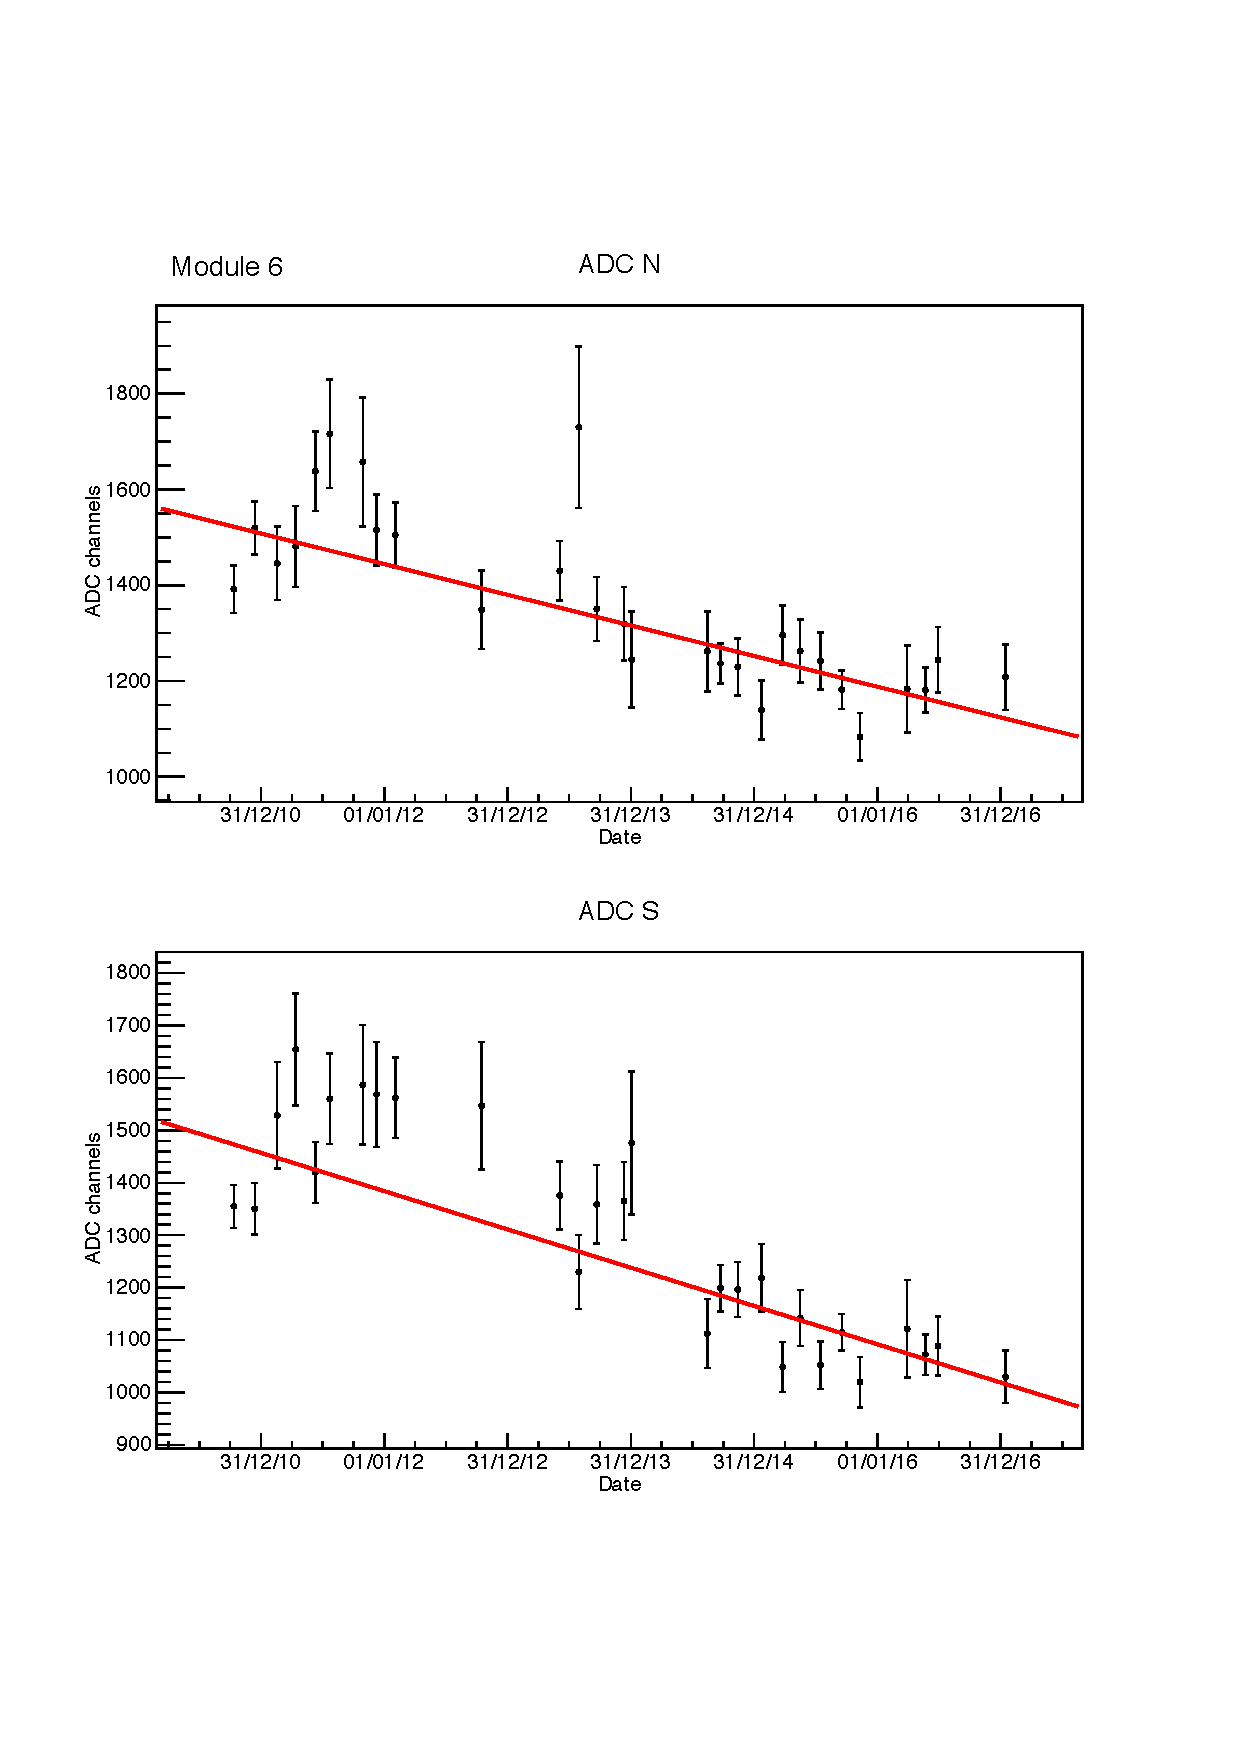
\includegraphics[width=\linewidth{}]{./fig/M6mpv.pdf}
    \caption{}
    \label{fig:MPV_M6}
  \end{subfigure}
  \begin{subfigure}{0.6\linewidth}
    \centering
    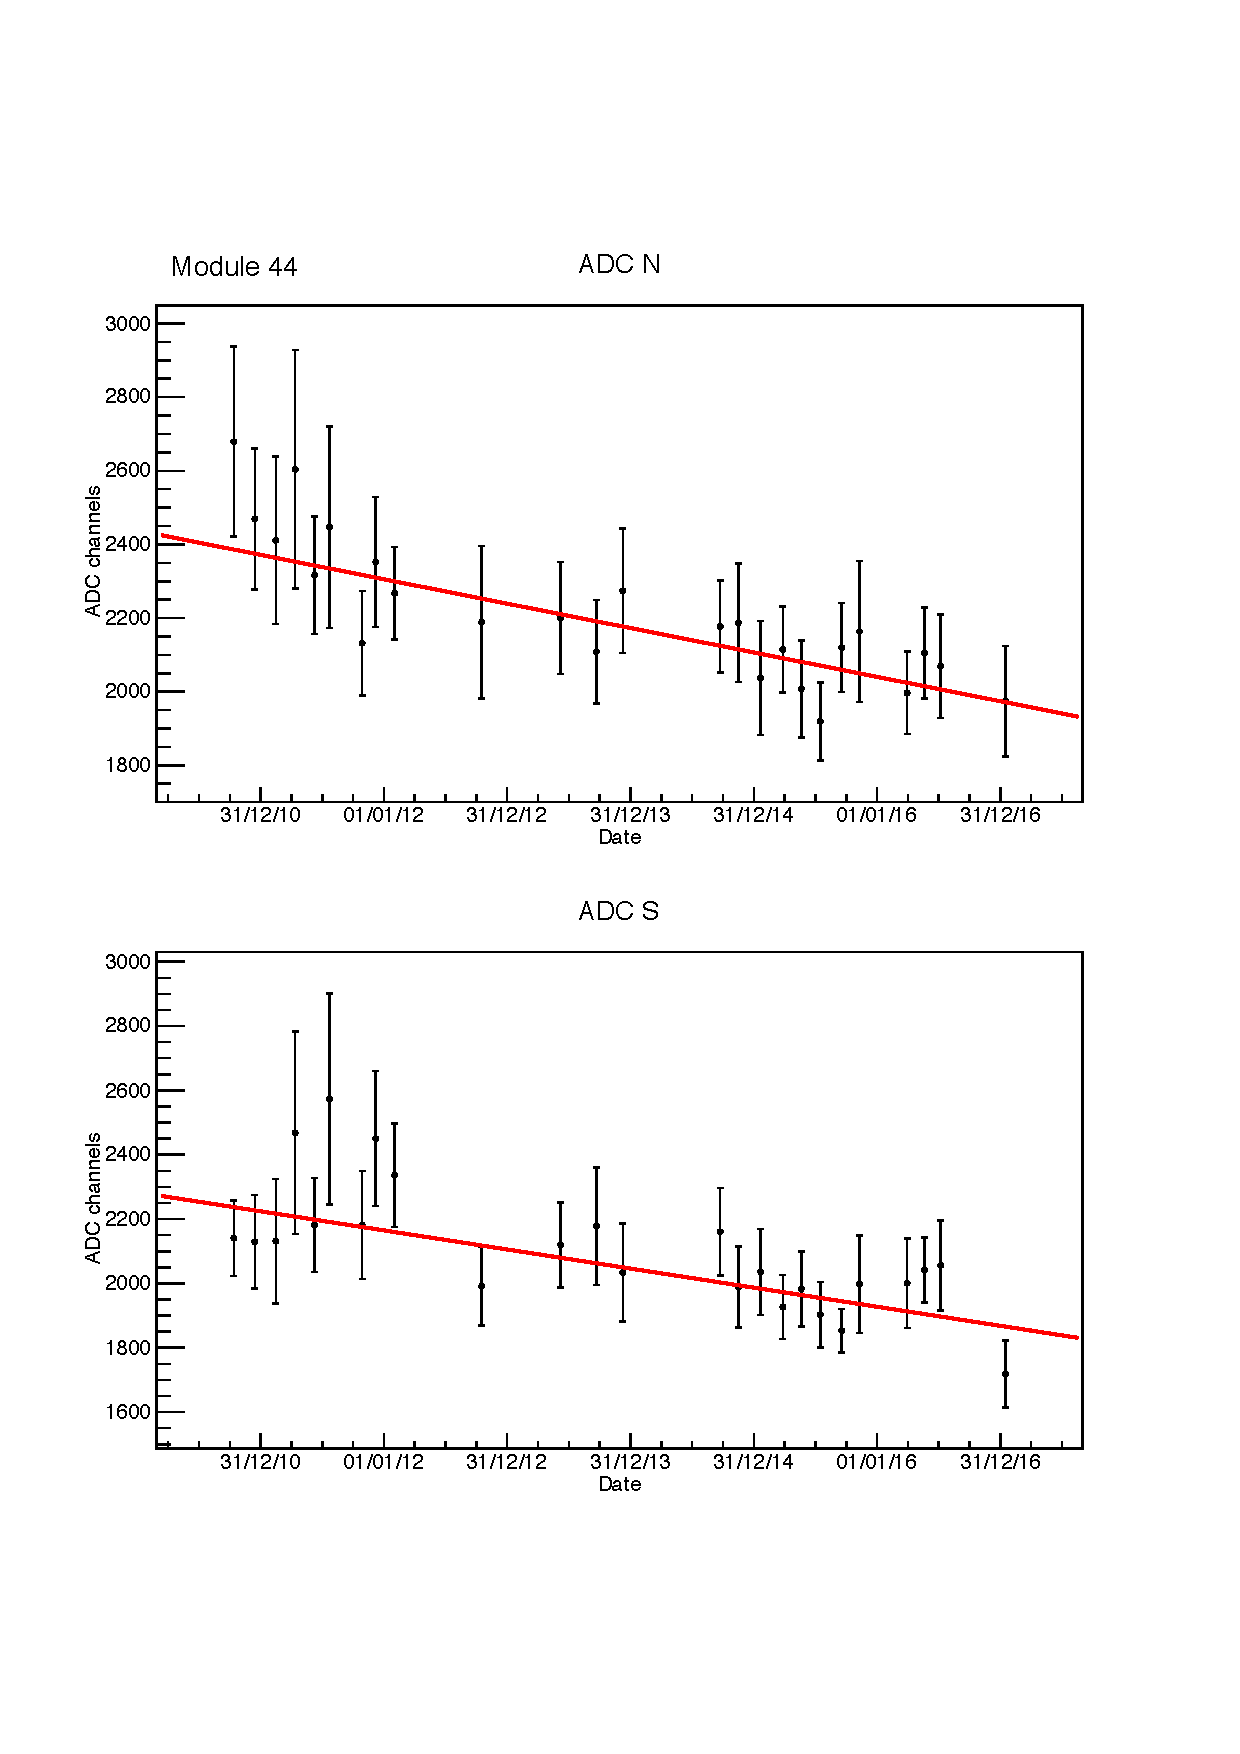
\includegraphics[width=\linewidth{}]{./fig/M44mpv.pdf}
    \caption{}
    \label{fig:MPV_M44}
  \end{subfigure}
  \caption{MPVs over time with linear fits in two example modules. The two upper figures show the MPVs in M6 (top module) and the two lower figures show the MPVs in M44 (bottom module). See \ref{tab:mpv} for values of the gradients.}
  \label{fig:MPV}
\end{figure}

%
%\begin{figure}[htb]
%  \centering
%  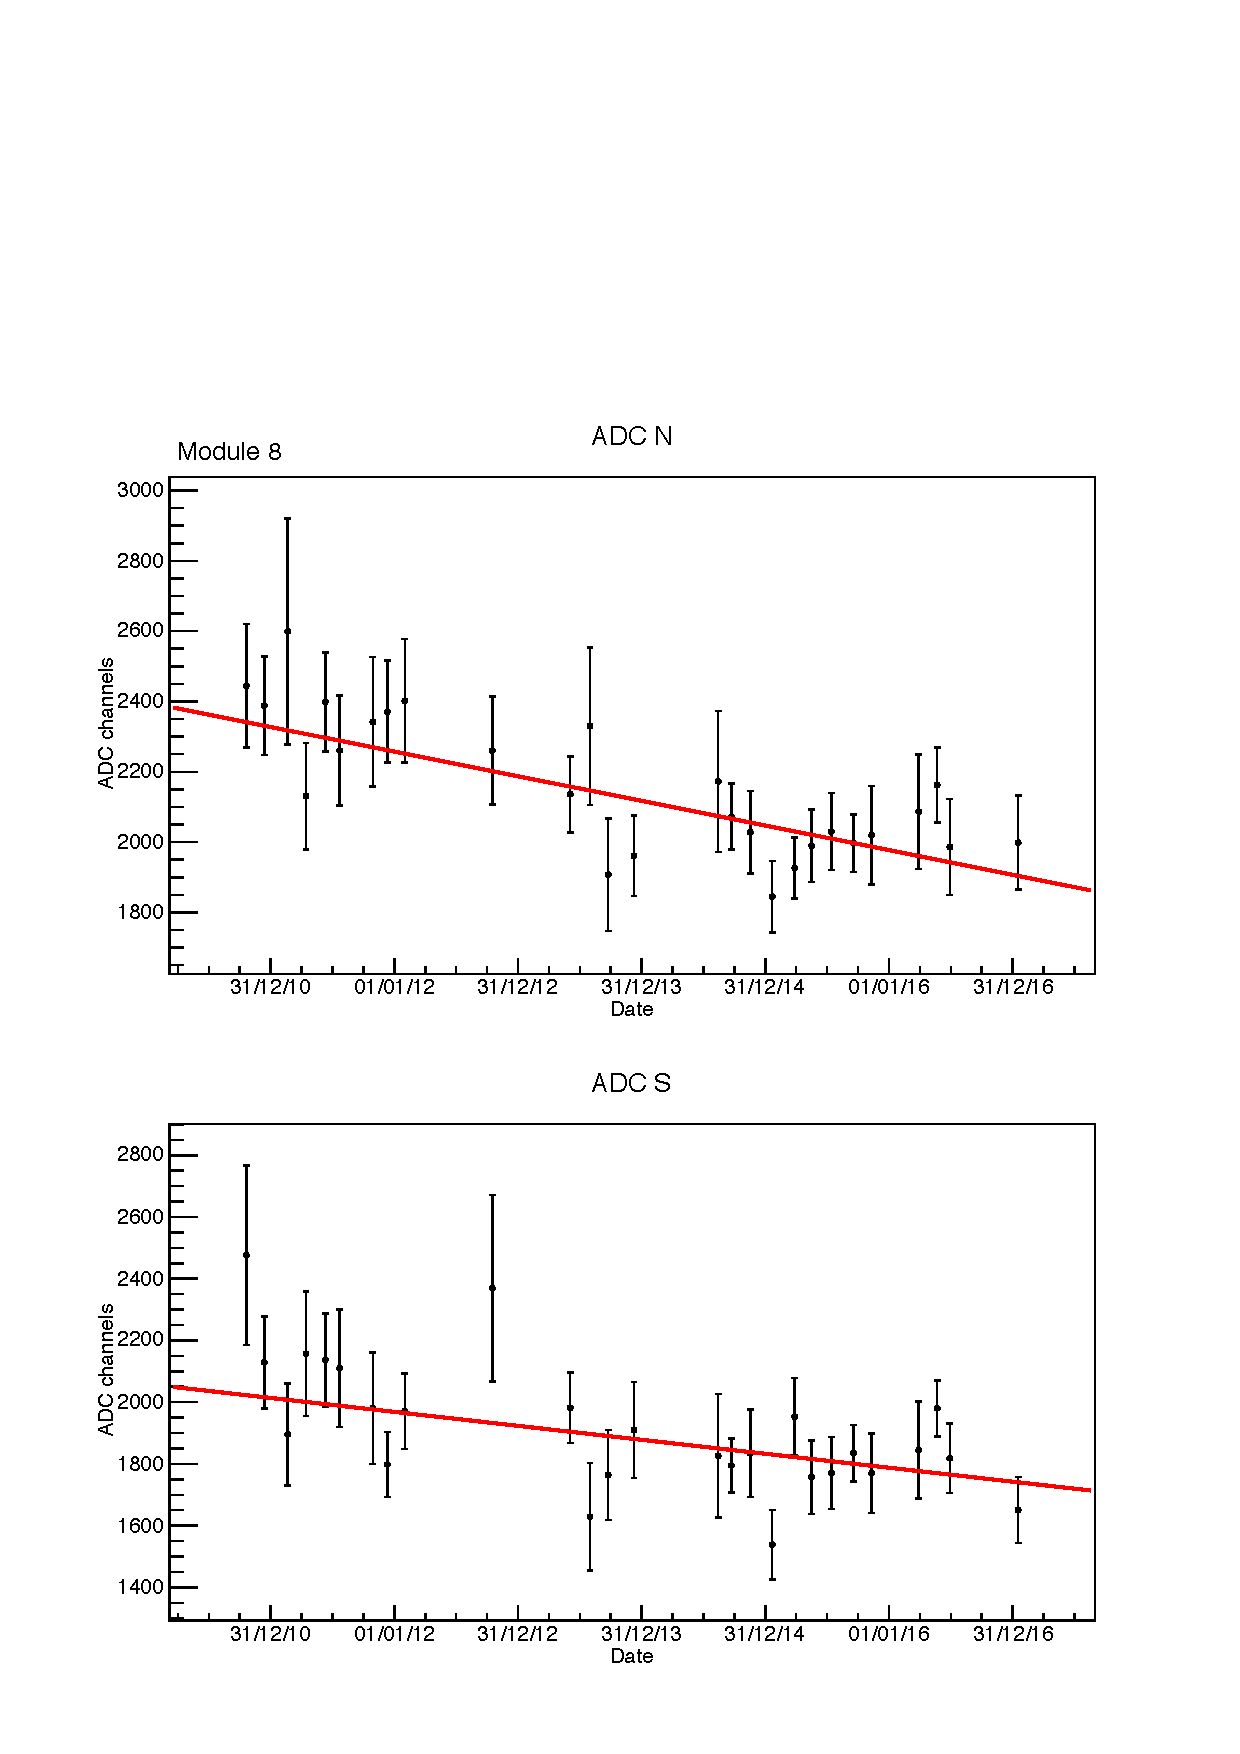
\includegraphics[width=0.6\textwidth{}]{./fig/M8mpv.pdf}
%  \caption{MPVs over time with linear fit in M8.}
%  \label{fig:Landau_M8}
%\end{figure}

\begin{table}[hb!]
  \centering
  \caption{Slopes of the linear regressions of MPVs in example modules M6, M8 and M44. The statistical uncertainty is obtained from the fit program in ROOT. }
  \label{tab:mpv}
  \begin{tabular}{c c c c}
  \toprule
  Module & \multicolumn{2}{c}{slope in channels/month} \\
         & ADC N & ADC S \\
  \midrule
  M6  & $-5.4\pm1.3$ & $-4.9\pm1.1$ \\
  M8  & $-5.3\pm0.5$ & $-6.0\pm0.5$ \\
  M44 & $-5.8\pm3.7$ & $-3.7\pm1.1$ \\
  \bottomrule
  \end{tabular}
\end{table}

The change of the MPVs are again approximated by a linear regression and the obtained slopes are listed in tab.\ \ref{tab:mpv}. It can be seen that the slopes for two ends in a single module don't vary much from each other, which means that the ageing of plastic scintillator is, as expected, almost symmetric and the electronics of two PMT groups may have also aged similarly.

The value obtained in M8 is also listed for comparison with the result from LED data $\Delta{}_{\mathrm{LED\,S}}=\SI{-4.2}{channels\per month}$ and $\Delta{}_{\mathrm{LED \,N}}=\SI{-1.8}{channels\per month}$. The decrease of the MPVs is larger than the one of ADC mean values of middle and northern LED events and lies in the uncertainty region of southern LED events. The abnormal increase of ADC mean values of LED S in M8 (see tab.\ref{tab:led}) is not found in the data obtained from muon events. Thus it can be concluded that the problem is merely due to the behaviour of the LED but not the scintillator module. \\
Despite the various effects that may lead to a sudden change of the ADC value, the MPVs of the Landau spectrum in all 46 modules show a general decrease of several hundred ADC channels since 2010.



\section{Determination of the detection efficiency}
The analysis above shows that the signal height recorded with the PMT groups has decreased remarkably since the start of the experiment. However, it doesn't provide a direct measure of the change of the muon detection efficiency. To estimate the detection efficiency, the knowledge of the trigger threshold of each module is needed. Before the experiment, the scintillator modules have been calibrated using cosmic muons \cite{Hab04}. Due to the ageing effects of the modules, the trigger threshold must be determined again. As the muon flux in the underground laboratory is reduced significantly, the cosmic muons cannot be used for calibration anymore. In this section, an alternative approach to determine the trigger threshold is described. The detection efficiencies in different time periods are derived using the obtained threshold values.

\subsection{Effective trigger threshold}
As discussed in section \ref{sec:muon-working}, there are two thresholds in the measurement of the \mvs{}. One is a digital conversion threshold, which is typically set to 120\,ADC channels. The influence of the digital threshold on the muon detection efficiency can be neglected, because the MPVs are typically above 1000\,ADC channels and the Landau distribution falls quickly towards the low energy region.

The trigger threshold, on the other hand, is relevant for the following analysis. It is a hardware threshold which is set to 150\,mV. Only pulses with an amplitude above this value trigger the data acquisition. Although the hardware threshold is set to the same voltage in each module, the value in ADC channels depends on the gain of the individual PMT groups. Thus the effective trigger threshold in term of energy deposit is individual for each module. \\
Additionally, it depends on the shape of measured pulse, as the ADC value is the integral of a signal. For example, a flat pulse has a larger energy deposit than a steep pulse with same amplitude. The pulse shape also depends on the light propagation and is thus position dependent. Thus, a calibration source would be needed to determine the position dependency of the trigger threshold, which is not performed in this work.

Averaging over the module length and taking the resolution into account, the effective trigger threshold is expected to be a curve instead of a step function. The efficiency of a module can be given as a function of energy, which is low for small energy deposit and is expected to be 100\% in the high energy region. It is similar to the behaviour of an error function:
\begin{equation}
  \mathrm{erf}(x)=\frac{2}{\sqrt{\pi}} \int_{0}^{x} \! e^{-t^{2}}\, \mathrm{d}t
\end{equation}
It describes the convolution of a Heaviside function $\Theta(x)$ with a Gaussian distribution. By shifting and rescaling, the error function is able to imitate the behaviour of the actual detection efficiency curve at the threshold. It is characterised by two parameters, the effective threshold $E_{\mathrm{thr}}$ and the standard deviation $\sigma$. The effective trigger threshold is defined as the ADC value where detection efficiency is 50\% and the $\sigma$ describes the smearing effect of the spectrum.

\subsubsection*{A Method to determine the effective trigger threshold}

When a module is triggered, all the non-zero signals in the \mvs{} are stored. It is therefore possible to analyse the the events for a certain module $i$ even if they don't trigger the module $i$. For the analysis of one PMT group X in module $i$, its ADC values of all the events, that have been triggered by a full coincidence in another module $j$, are stored in histogram H1. In contrast to the condition of muon selection, which requires both non-zero TDC values, the trigger condition of the PMT group X used in the following analysis requires only that the TDC on the same side has a non-zero value. Requiring both TDC channels will introduce a dependency on the PMT group on the other side, while the trigger threshold is determined separately for two ends of a module. The events with a non-zero TDC value, i.e.\, have passed the threshold, are stored in histogram H2. The trigger efficiency of the PMT group X is determined by the division of H2 and H1.

\begin{figure}[ht]
  \centering
  \begin{subfigure}{0.7\linewidth}
    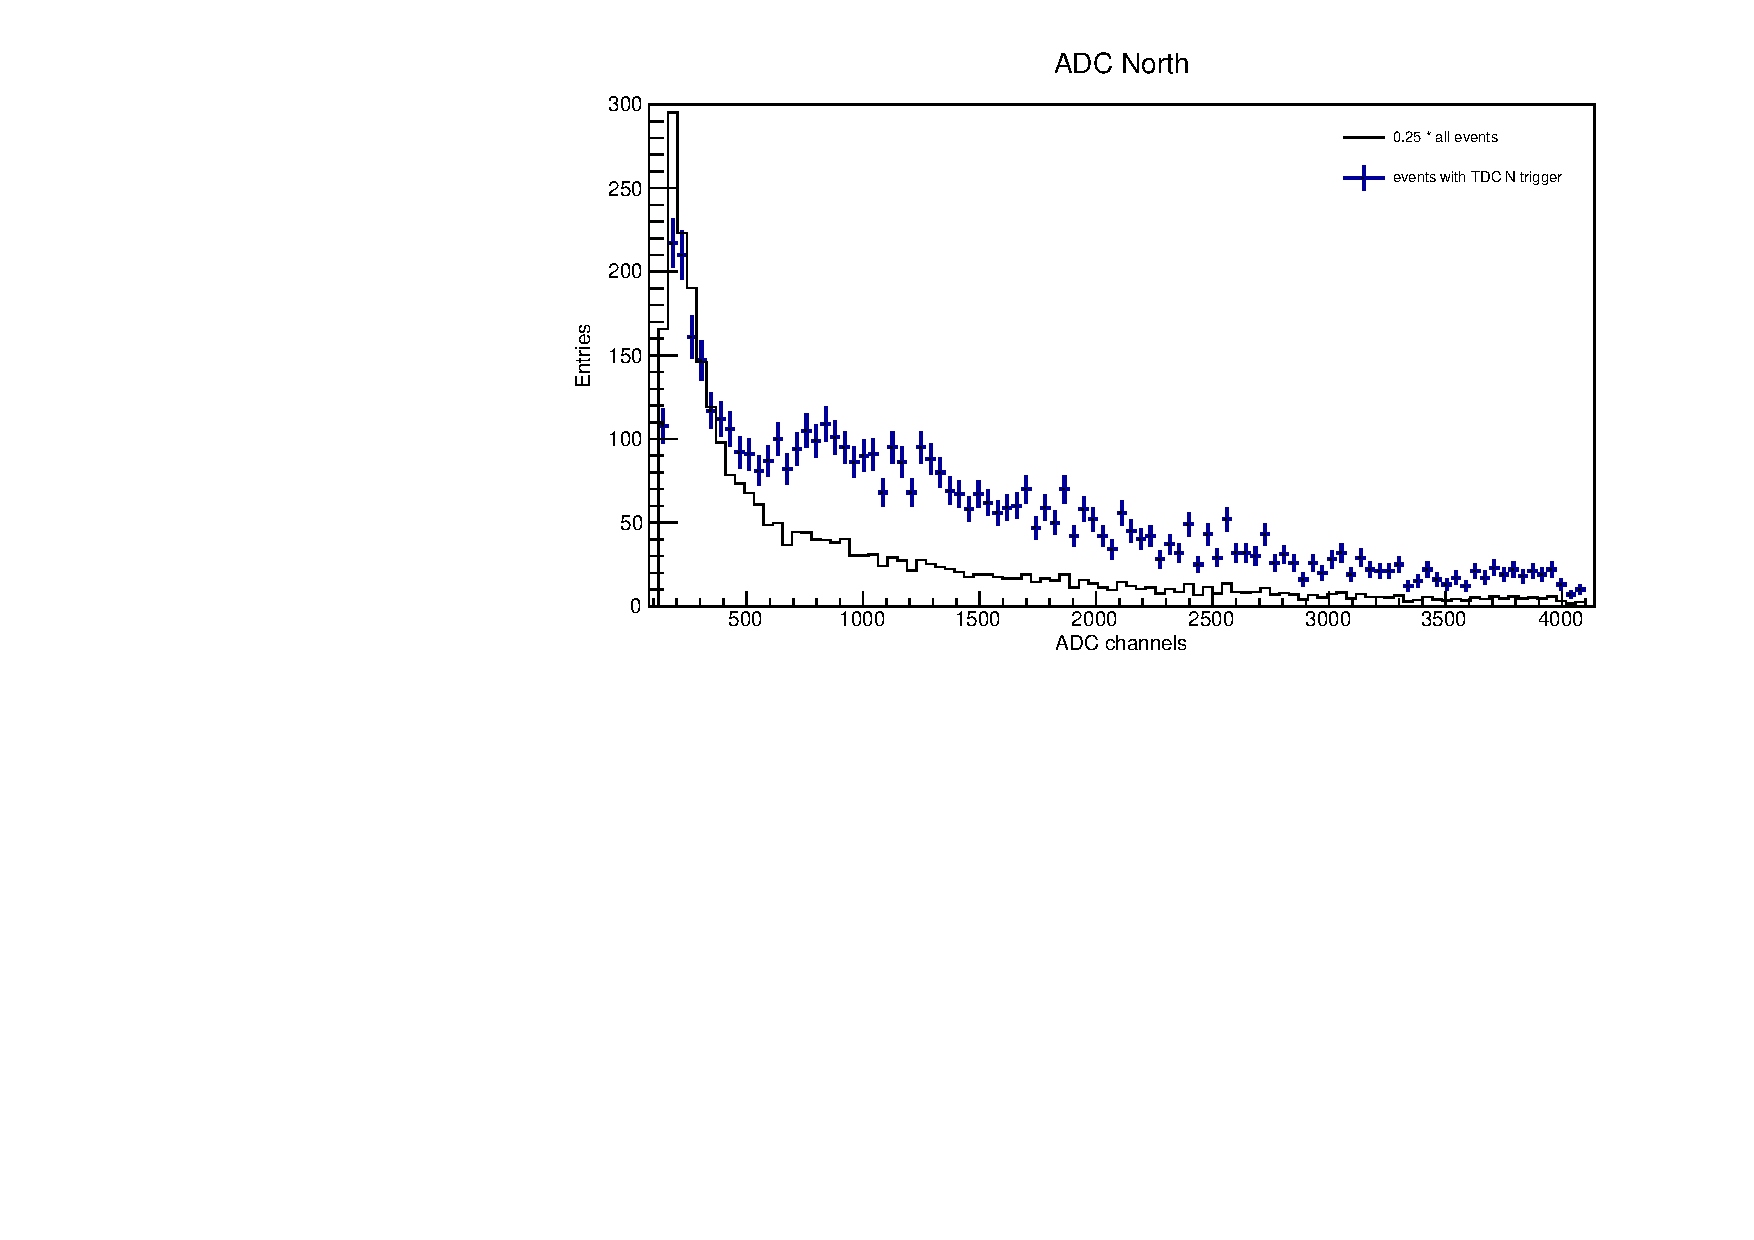
\includegraphics[width=\linewidth{}]{./fig/M6AdcNorth2Histo.pdf}
    \caption{Example of the spectrum with and without trigger condition of ADC N in M6. The data points (blue) are events which satisfy the trigger condition in the same end (Northern PMT group). The spectrum of all events (black) are scaled by a factor of 4.}
    \label{fig:2HistoM6}
  \end{subfigure}
  \begin{subfigure}{0.7\linewidth}
    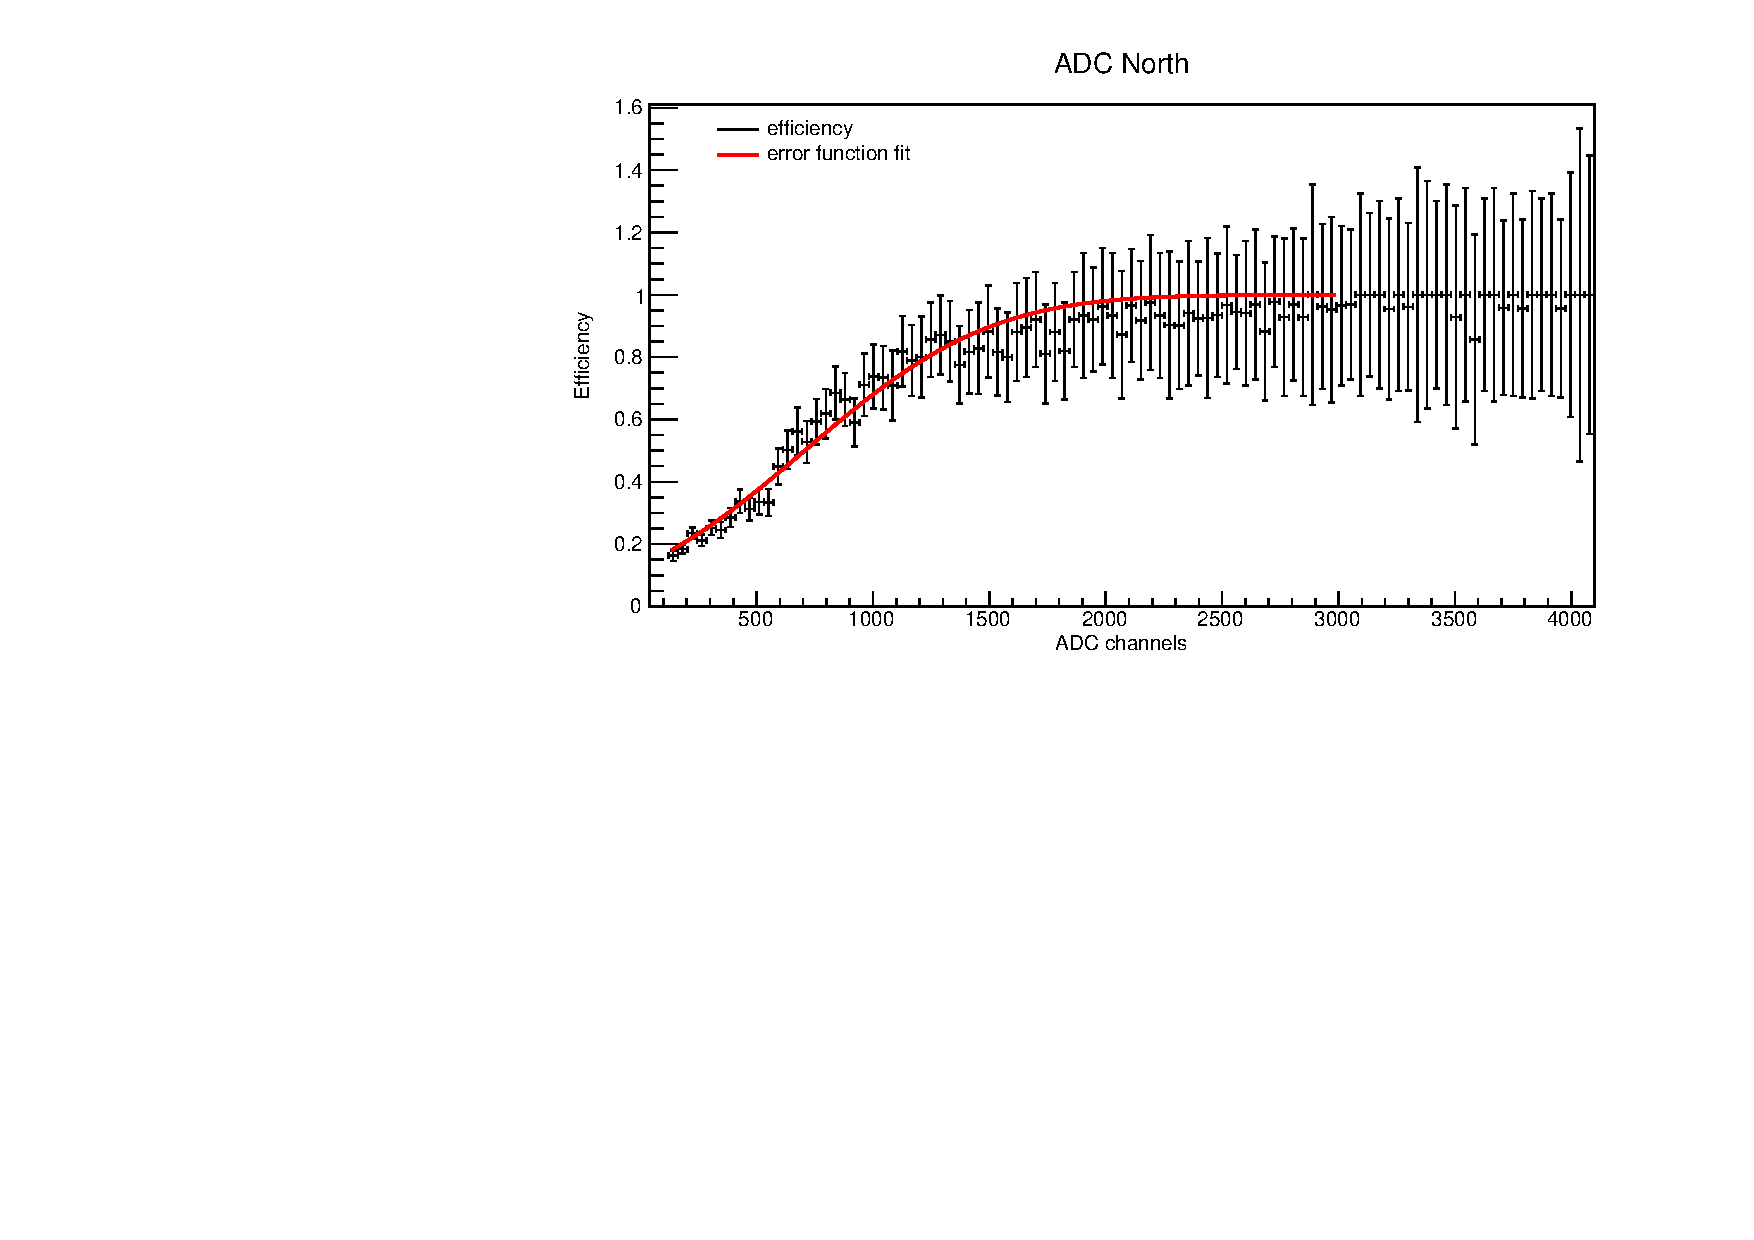
\includegraphics[width=\linewidth{}]{./fig/M6AdcNortheff_late.pdf}
    \caption{Histogram of events triggering the PMT group on the same side divided by all events with error bars (black) and the error function fit (red).}
    \label{fig:eff_lateM6}
  \end{subfigure}
  \caption{Method to determine the effective trigger threshold of a PMT group exemplified for ADC North of Module 6.}
  \label{fig:threshold_example}
\end{figure}

Fig.\,\ref{fig:threshold_example} shows an example of this method using the events in Module 6. The events that triggered one PMT group are plotted with all events. As expected, the detection efficiency increases with ADC values and goes toward 100\%. As can be seen in the figure, the increase is slightly asymmetric: it is more rapid at first and is then flatter. The estimation with an error function is therefore conservative for rather small energy deposits and optimistic for higher energy events.

The effective trigger threshold in ADC units are calculated for each PMT group in different time periods. To increase statistics, several runs are combined to perform the error function fit. Run 70-79 (year 2010) are investigated for the early time period and Run 124-138 (year 2015-2017) for the late time period. The results are listed in tab.\,\ref{tab:efficiency_short} in the following section.


\subsection{Detection efficiency of a module}
In addition to the above criteria, events with a coincidence in adjacent modules are excluded. These events have a higher probability to be induced by secondary particles or grazing muons. They mostly have small energy deposits, where the efficiency is also small due to the trigger threshold, and can lead to a decrease of the derived total detection efficiency.

\begin{figure}[h!]
  \begin{subfigure}{0.5\linewidth}
    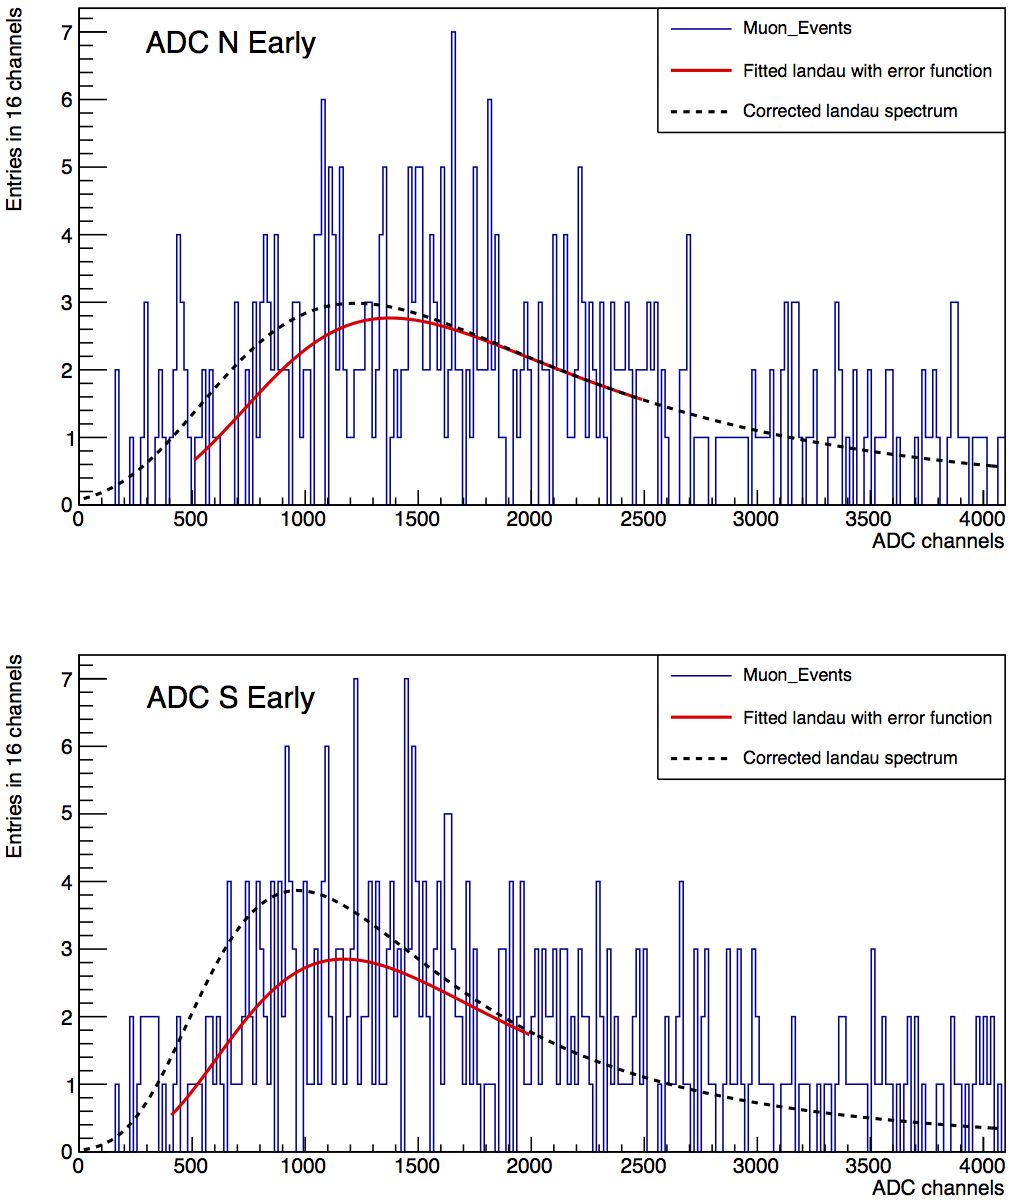
\includegraphics[width=\linewidth{}]{./fig/70M6CorrectedLandau.png}
  \end{subfigure}
  \begin{subfigure}{0.5\linewidth}
    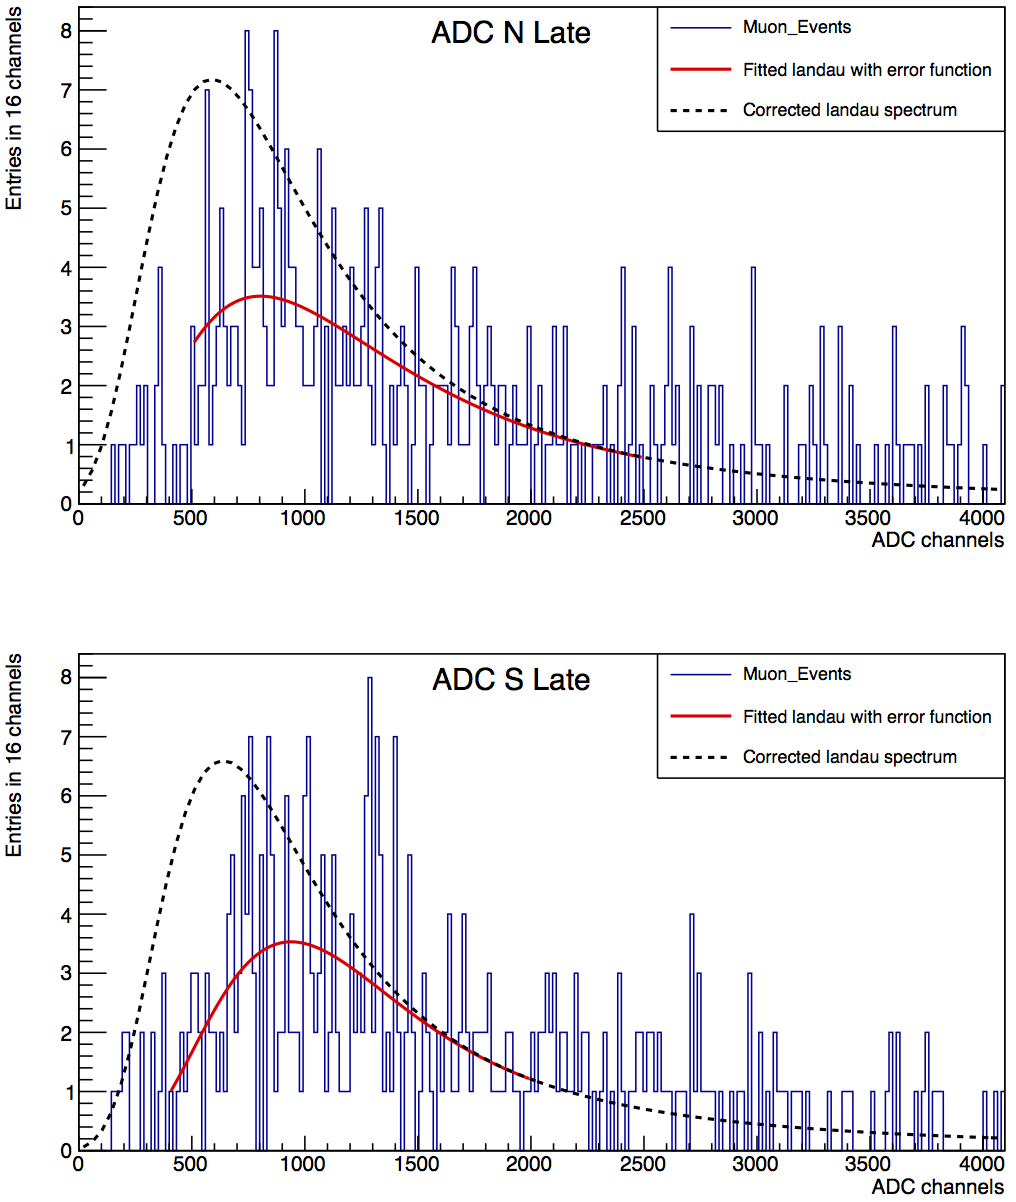
\includegraphics[width=\linewidth{}]{./fig/124M6CorrectedLandau.png}
  \end{subfigure}
  \caption{Spectrum of muon-induced events in M6 in earlier runs (left) and latest runs (right). The spectra are fitted with a Landau distribution with an error function (red). The corrected spectrum (black, dotted) is determined by dividing the error function.}
  \label{fig:detection_M6}
\end{figure}

The muon energy deposit can be described with a Landau distribution, whereas the measured energy deposit is dependent on the response of the individual modules. Therefore, the ADC spectrum is expected to be a Landau distribution multiplied by an error function. The parameters of the error function are calculated above in the determination of the effective trigger threshold. The selected data are fitted with this function and the corrected spectrum is given by a Landau distribution with the obtained parameters from the fit (see fig. \ref{fig:detection_M6}). The efficiency can be determined by the integral of the spectrum with and without the error function.


\begin{table}[htb!]
  \caption{The trigger threshold and detection efficiency of PMT groups in selected modules on different sides of the \mvs{} (for the full table see appendix \ref{sec:appendix}). The MPV in this table denotes the most probable value of the Landau distribution. Parameters of the error function are given as Threshold and $\sigma{}_{\mathrm{erf}}$. The total efficiency is estimated via the product of the efficiency value $\epsilon_{50\%\mathrm{MPV}}$ of each PMT group, which is determined by the integration from half of the MPV energy (See text for more details). For M15, see also fig.\,\ref{fig:fail_M15}.}
  \label{tab:efficiency_short}
  \begin{tabular}{c c c c c c c c c}
    \toprule
    Module & End & MPV & Threshold & $\sigma{}_{\mathrm{erf}}$ & $\epsilon_{20\%}$ & $\epsilon_{50\%\mathrm{MPV}}$ & $\epsilon_{\mathrm{MPV}}$ & $\epsilon_{\mathrm{tot}, 50\%\mathrm{MPV}}$ \\
           &     & \multicolumn{3}{|c|}{in ADC channels} &   \\
    \midrule
    M6     & N & 1401 & 532 & 737 & 0.86 & 0.90 & 0.97 & \multirow{2}{*}{0.77}\\
    early  & S & 1256 & 615 & 712 & 0.83 & 0.86 & 0.95 &\\
    M6     & N & 872 & 707 & 627 & 0.67 & 0.71 & 0.85 & \multirow{2}{*}{0.53}\\
    late   & S & 975 & 746 & 416 & 0.60 & 0.75 & 0.94\\
    \midrule
    M15    & Nemo & 2674 & 560 & 143 & 0.99 & 1.00 & 1.00 & \multirow{2}{*}{1.00}\\
    early  & Est & 1292 & 186 & 13 & 1.00 & 1.00 & 1.00\\
    M15    & Nemo & 1713 & 1879 & 758 &  &  &  & \multirow{2}{*}{0.59}\\
    late   & Est & 1284 & 958 & 280 & 0.73 & 0.77 & 0.99 & \\
    \midrule
    M17    & B & 1200 & 515 & 112 & 0.99 & 1.00 & 1.00 & \multirow{2}{*}{0.94}\\
    early  & H & 1043 & 100 & 740 & 0.88 & 0.94 & 0.98 &\\
    M17    & B & 1457 & 855 & 384 & 0.82 & 0.90 & 0.99 & \multirow{2}{*}{0.80} \\
    late   & H & 1359 & 671 & 611 & 0.72 & 0.89 & 0.98 & \\
    \midrule
    M36    & Est & 1452 & 912 & 803 & 0.61 & 0.80 & 0.93 & \multirow{2}{*}{0.67} \\
    early  & Nemo & 1346 & 821 & 568 & 0.79 & 0.83 & 0.96 &\\
    M36    & Est & 1201 & 1114 & 624 & 0.48 & 0.62 & 0.85 & \multirow{2}{*}{0.45}\\
    late   & Nemo & 1373 & 1060 & 531 & 0.61 & 0.72 & 0.93 & \\
    \bottomrule
  \end{tabular}
\end{table}

However, integrating the total histogram starting from 0 will not give a reliable result. As the efficiency falls to 0 in low energy regions, this low-statistics part of the corrected spectrum will have large contribution and significantly reduce the total efficiency. Additionally, the fraction of muons with energy deposit well below the MPV is expected to be low in reality. Therefore, it is reasonable to integrate the spectrum from a certain energy value.\\
Three efficiency values with different integration start points are given for each PMT group. $\epsilon_{20\%}$ integrates from the energy where the entries are equal to 20\% of the entries at MPV. $\epsilon_{\mathrm{MPV}}$ integrates from the MPV and gives an optimistic estimation. Therefore, the total efficiency of a module is given by the product of $\epsilon_{50\%\mathrm{MPV}}$ in two PMT groups, for which the spectrum is integrated from half of the energy at MPV. The results for selected modules are listed in tab.\,\ref{tab:efficiency_short}, the complete table is given in appendix \ref{sec:appendix}.

For some of the PMT groups, the spectrum cannot be fitted properly (for an example see fig.\,\ref{fig:fail_M15}). The efficiency is estimated by the other PMT group in the same module. If the fit method cannot be applied for both PMT groups, the total detection efficiency is given by the mean values of other modules on the same side.


\begin{figure}[ht!]
  \centering
  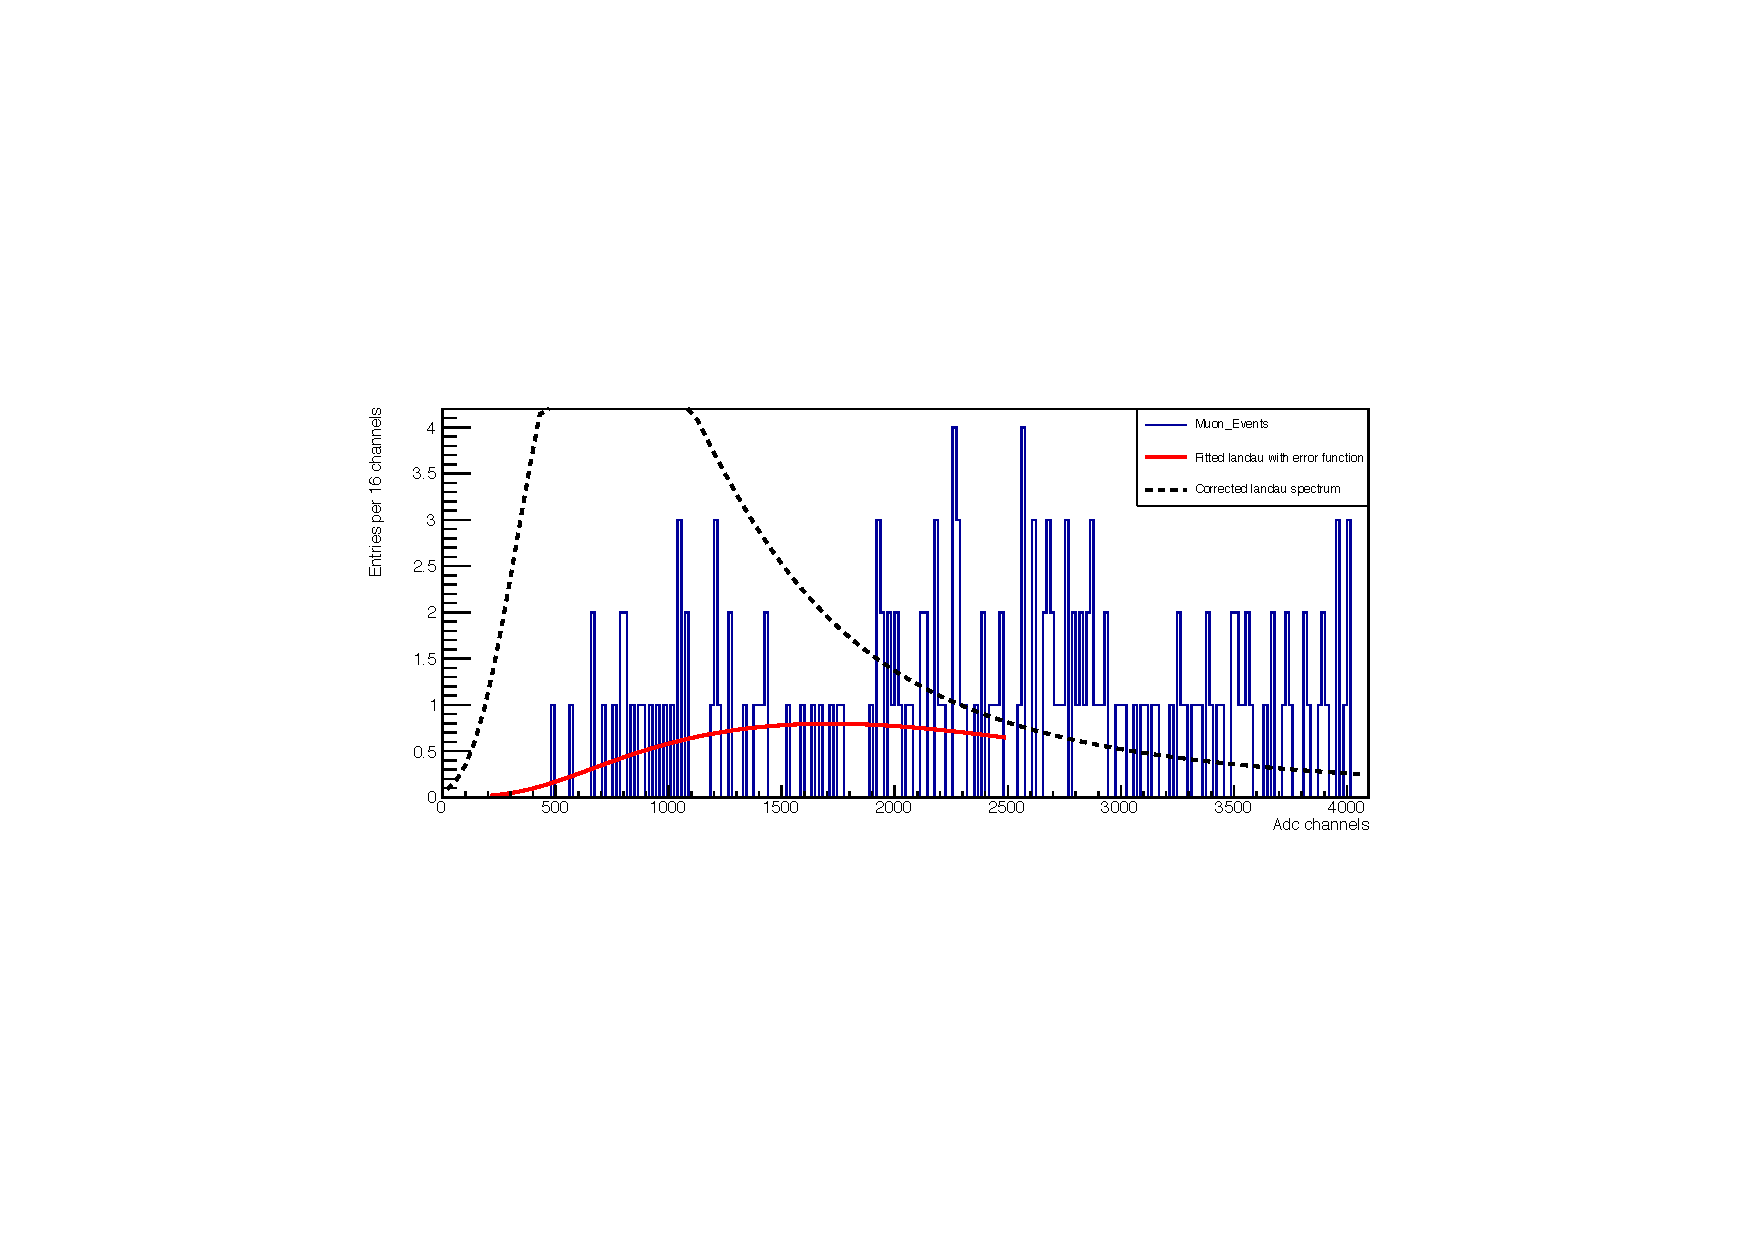
\includegraphics[width=0.7\textwidth{}]{./fig/M15fail.pdf}
  \caption{Example of a failed fit of PMT Nemo in M15 in Run124-138. The efficiency is given by the other PMT group in the same module.}
  \label{fig:fail_M15}
\end{figure}

As expected, the MPV decreased and the effective trigger threshold increased in the time period of seven years, which lead to a loss of detection efficiency. Most modules show a relative decrease of about 30\%. Although the relative change is significant, the absolute values of detection efficiency should only be used as lower limits, since they are strongly underestimated as discussed below. An analysis in 2010 using a similar method obtained the result $\epsilon_{\mathrm{M6}}=0.88$ and $\epsilon_{\mathrm{M36}}=0.96$ \cite{Nie10}, showing that the efficiency values derived here are indeed too conservative.

The underestimation results from the following facts. First of all, there are still contributions of secondary particles or backgrounds to the low energy region despite the cuts applied. The obtained MPVs derived from the fit are thus smaller and it leads to a smaller detection efficiency.

Secondly, the gain of two PMT groups are considered as uncorrelated for the matter of simplification, while they are correlated in reality. As shown in section \ref{sec:muon-working}, the light yield measured in the near PMT group is larger than the one in the far PMT group. This leads to an overestimation for near end and underestimation for far end. Since the efficiency decreases drastically in the low energy region, the total detection efficiency is expected to be underestimated. However, the effect of correlation cannot be implemented due to the low statistics of muon events.

%why is eff so low

Additionally, the muons passing through the \mvs{} have a second chance to be detected when leaving the system. Also, they can partly be detected by measuring the particle showers. Last but not least, the grazing muons, which go through adjacent modules and deposit energy well below MPV, are possible to be detected in both modules. To conclude, the absolute value of detection efficiency derived here should be treated as lower limit and the total efficiency of the \mvs{} is higher than the one of individual modules.

%The result shows that the detection efficiency for most of the modules has decreased significantly. Despite that the rate of $\upmu{}$-induced WIMP-like signals is estimated to be low, it can limit the sensitivity of WIMP search if the efficiency of \mvs{} drops. To retain a high detection efficiency as the start of the experiment, the HV applied on individual PMT groups should be increased. By doing so, the gain of PMT groups increases, corresponding to a higher MPV in ADC units and lower effective threshold.

\subsection{Conclusion and comparison to earlier works}
In this chapter, the effective trigger threshold of each PMT group is determined. The detection efficiency of individual modules is derived using the selected muon events and the obtained threshold parameters. With the obtained detection efficiency of a single module, the probability for a muon going through 2 modules to be detected by the \mvs{} can be given as
\begin{equation}
  P_{\mathrm{total}}=\frac{1}{2}\cdot \sum\limits_{i} \left( P_{\mathrm{geo,i}}\cdot P_{i} +(1-P_{\mathrm{geo,i}}\cdot P_{i})\cdot \sum\limits_{j\ne i} P_{\mathrm{geo,ij}\cdot P_{j}}  \right)-P_{\mathrm{gap}},
\end{equation}
where $P_{i}$ is the detection efficiency of a single module $i$. Since the direction of muons are not equally distributed, the normalised probability that a muon goes through the module $i$ is given by $P_{\mathrm{geo,i}}$. $P_{\mathrm{geo,ij}}$ denotes the probability that the muon goes through both modules $i$ and $j$. Also, there is a small probability that a muon goes through the gap of the \mvs{}, which is given by $P_{\mathrm{gap}}$. \\
However, the detection efficiency of the total \mvs{} is not derived as the geometric coefficients are not available for this work. These parameters can be determined by a simulation of the muon flux and then the total detection efficiency can be caculated using the above equation. \\
Here, an example of the combined detection efficiency of two modules is described. Consider a muon going through M6 (top) and M46 (bottom), which probably hits the bolometers and can potentially induce a neutron signal. The detection efficiencies of M6 and M46 in early and late stage are
\begin{align}
  \epsilon_{6,\mathrm{early}} &= 0.77 & \epsilon_{6,\mathrm{late}} &= 0.53 \\
  \epsilon_{46,\mathrm{early}} &= 0.58 & \epsilon_{6,\mathrm{late}} &= 0.38.
\end{align}
Thus the probabilities that the muon is detected in both modules are
\begin{align}
  \epsilon_{6+46,\mathrm{early}} &= 0.89 \\
  \epsilon_{6+46,\mathrm{late}} &= 0.74.
\end{align}

The relative change of detection efficiency using combination M6 and M46 is thus 17\%. It it also expected that the change of the detection efficiency of the \mvs{} is smaller than the change of a single module. \\
The total detection efficiency of the \mvs{} was determined in 2010 to be $\epsilon_{\mathrm{total}} \geq 0.949$ using a similar method \cite{Nie10}. Therefore, as discussed before, the result obtained here gives a reliable lower limit on the actual value.

It should be mentioned that the detection efficiency of the \mvs{} can also estimated using different methods. For example, coincidences between the \mvs{} and the bolometers can be studied. As the muon-induced bolometer events can be distinguished from other backgrounds by their multiplicity and energy deposit, these events can be selected. The detection efficiency can thus be derived by searching for the coincidences in the \mvs{} in a certain time window. The detection efficiency of the \mvs{} is determined to be $\epsilon_{\mathrm{total}} \geq 0.93$ (90\% C.L.) in 2015 \cite{Kef16}.

It can be concluded that the detection efficiency for most of the modules has decreased significantly and the obtained value gives a lower limit on the actual value. The relative change of the detection efficiency is still significant.
Despite that the rate of $\upmu{}$-induced WIMP-like signals is estimated to be low, it can limit the sensitivity of WIMP search if the efficiency of the \mvs{} drops. \\
To retain a detection efficiency as high as at the start of the experiment, the HV applied on individual PMT groups should be increased. By doing so, the gain of PMT groups increases, corresponding to a higher MPV in ADC units and lower effective threshold. However, the decrease of the detection efficiency cannot be infinitely compensated by a higher HV, as the applied HV has an upper limit.\\
As mentioned before, the 46 scintillator modules were previously used in the KARMEN experiment and have an age over 20 years \cite{Rei98}. The analysis above shows that almost all of them have aged significantly over the last 7 years. Although they have shown a sufficient performance during the EDELWEISS experiment, they are not suitable to be used as a muon shielding for upgrades or further experiments requiring a higher sensitivity.






%blahblah
